\documentclass[12pt]{article}

\usepackage{amsmath,amsfonts,amsthm,amssymb}
\usepackage{color}
\usepackage{graphicx}
\usepackage{wrapfig}
\usepackage{epsfig}
%\usepackage{subfigure}
\usepackage{times}
\usepackage{xspace}
\usepackage{url}
\usepackage{pdfpages}
\usepackage{array}
\usepackage{subfig}
\usepackage{multirow}
\usepackage{dblfloatfix} 

\setlength{\topmargin}{0.0in}     % top of paper to head (less one inch)
\setlength{\headheight}{0in}      % height of the head
\setlength{\headsep}{0in}         % head to the top of the body
\setlength{\textheight}{9.0in}    % height of the body
\setlength{\oddsidemargin}{-.25in} % left edge of paper to body (less one inch)
\setlength{\evensidemargin}{0mm}  % ditto, even pages
\setlength{\textwidth}{7.0in}     % width of body
\setlength{\topskip}{0in}         % top of body to bottom of first line of text
\setlength{\parindent}{1pc}       

\begin{document}
\thispagestyle{empty}
%%%%%%%%%%%%%%%%%%%%%%%%%%%%%%%%%%%%%%%%%%%%%%%%%%%%%%%%%%%%%%%%%%%%%%%%%%%%%%%%%%%%%%%%
% Project Summary
%%%%%%%%%%%%%%%%%%%%%%%%%%%%%%%%%%%%%%%%%%%%%%%%%%%%%%%%%%%%%%%%%%%%%%%%%%%%%%%%%%%%%%%%
\begin{center}
{\Large\bf Assignment \#5: Experimenting with color}
\vspace{3mm}
\\Caitlin Ross 
\\02/25/2016
\\*[3mm]
\end{center}
%%%%%%%%%%%%%%%%%%%%%%%%%%%%%%%%%%%%%%%%%%%%%%%%%%%%%%%%%%%%%%%%%%%%%%%%%%%%%%%%%%%%%%%%
% Task Objects
%%%%%%%%%%%%%%%%%%%%%%%%%%%%%%%%%%%%%%%%%%%%%%%%%%%%%%%%%%%%%%%%%%%%%%%%%%%%%%%%%%%%%%%%
\section{Chosen Visualization}
For this assignment, I chose to continue working on my parallel coordinates visualization of simulation data.  For comparison purposes, the original can be found at \url{https://caitlinross.github.io/vis/parcoords.html} and the improved version can be found at \url{https://caitlinross.github.io/vis/parcoords2.html}.  The changes for this week include, using a new simulation model for input data, addition of checkboxes so the user can choose which axes to view, and 16 different color palettes.  

\section{Data Source (ROSS)}
%Description of the data source and corresponding applications.
Again, I'm using the
ROSS parallel discrete-event simulator that
can process billions of events per second \cite{Holder}, \cite{Bauer}. ROSS
models are made up of a collection of logical processes (LPs).
Each LP models a distinct component of the system. LPs
interact with one another through events in the form of time-stamped messages. An MPI task is abstracted as a processor
element (PE) in ROSS. Each PE owns a number of LPs and
schedules events in time-stamp order for all LPs assigned to
it. Events that are destined for a logical process on another
PE (i.e. remote events) are sent as MPI messages. 

For parallel execution, ROSS uses an optimistic synchronization protocol.  When an LP determines it has processed events out of timestamp order, it rolls back event computation and re-executes events in the correct order.  The Global Virtual Time (GVT) is computed on a regular basis, which allows for a reclamation of events with timestamps smaller than GVT.  The ROSS scheduler computes GVT every \texttt{gvt\_interval} iterations in the scheduling loop.  Another variable \texttt{batch} can be set to determine the number of events processed during each iteration of the scheduling loop, so \texttt{gvt\_interval$*$batch} events are processed between successive GVT computations.  Changing these parameters can trigger large changes in metrics such as number of reverse computations, remote events, event efficiency, etc. Currently, the only data collection is averaged over all processes and collected at the very end of the simulation. Noah Wolfe and I made changes to the ROSS repo last week that collects data for each metric after certain GVT calculations throughout a simulation. 


\section{Data Format, Extraction \& Manipulation} 
%With your research questions in mind, design the detailed format for your raw data (the columns of your data "spreadsheet") and decide on the action or sampling frequency for each "row" of the data. Make sure you are able to acquire an "interesting" amount of data, both number of samples (at least 1000 rows?) and dimensions per sample (at least 3 columns?) Note: These estimates are not requirements. If your data has many more columns, things can be quite interesting even with far fewer rows.
%Detail the efforts you made to collect, parse, reorganize, simplify, and/or post-process this data source.
I collected data in the same format as last week's assignment.  I ran the Dragonfly network model with 8 MPI ranks.  I again varied the \texttt{batch} and \texttt{gvt\_interval} parameters for the runs.  For the experiments where \texttt{batch} is held constant, \texttt{batch=2} and \texttt{gvt\_interval} varies from 16 to 4096 by powers of 2.  This results in 329 rows of data.  For the experiments where \texttt{gvt\_interval} is held constant, \texttt{gvt\_interval=1024} and \texttt{batch} varies from 2 to 128 by powers of 2.  This results in 16,544 rows of data.  I combined the files from each run and PE into one file each for the \texttt{batch} (alldata-batch.csv) and \texttt{gvt\_interval} (alldata-gvt.csv) runs.  The experiments performed here result in approximately 253,000 data points for all of the data.


\section{Non-color Improvement}
%Create (at least 2) simple visualization plots of this data using a tool that's new to you (or you would like to learn more about). Consider using: Excel, LineUp, Tableau, Google Analytics, Plotly, or VTK. These plots should attempt to answer the research questions you posed earlier. You can revise your research questions as needed as you work with the data.
There are two non-color improvements that I made.  The first one is related to the idea of Focus + Context visualization introduced in~\cite{Hauser}.  Previously when selecting a subset of data on an axis in my visualization, all other lines disappeared.  Now they are simply greyed out in order to provide some context to the subset of data being viewed in more detail.  This was a fairly simple adjustment to make using the parcoords.js library~\cite{Chang}.

\section{Color Schemes}
\begin{figure}[ht]
\centering
	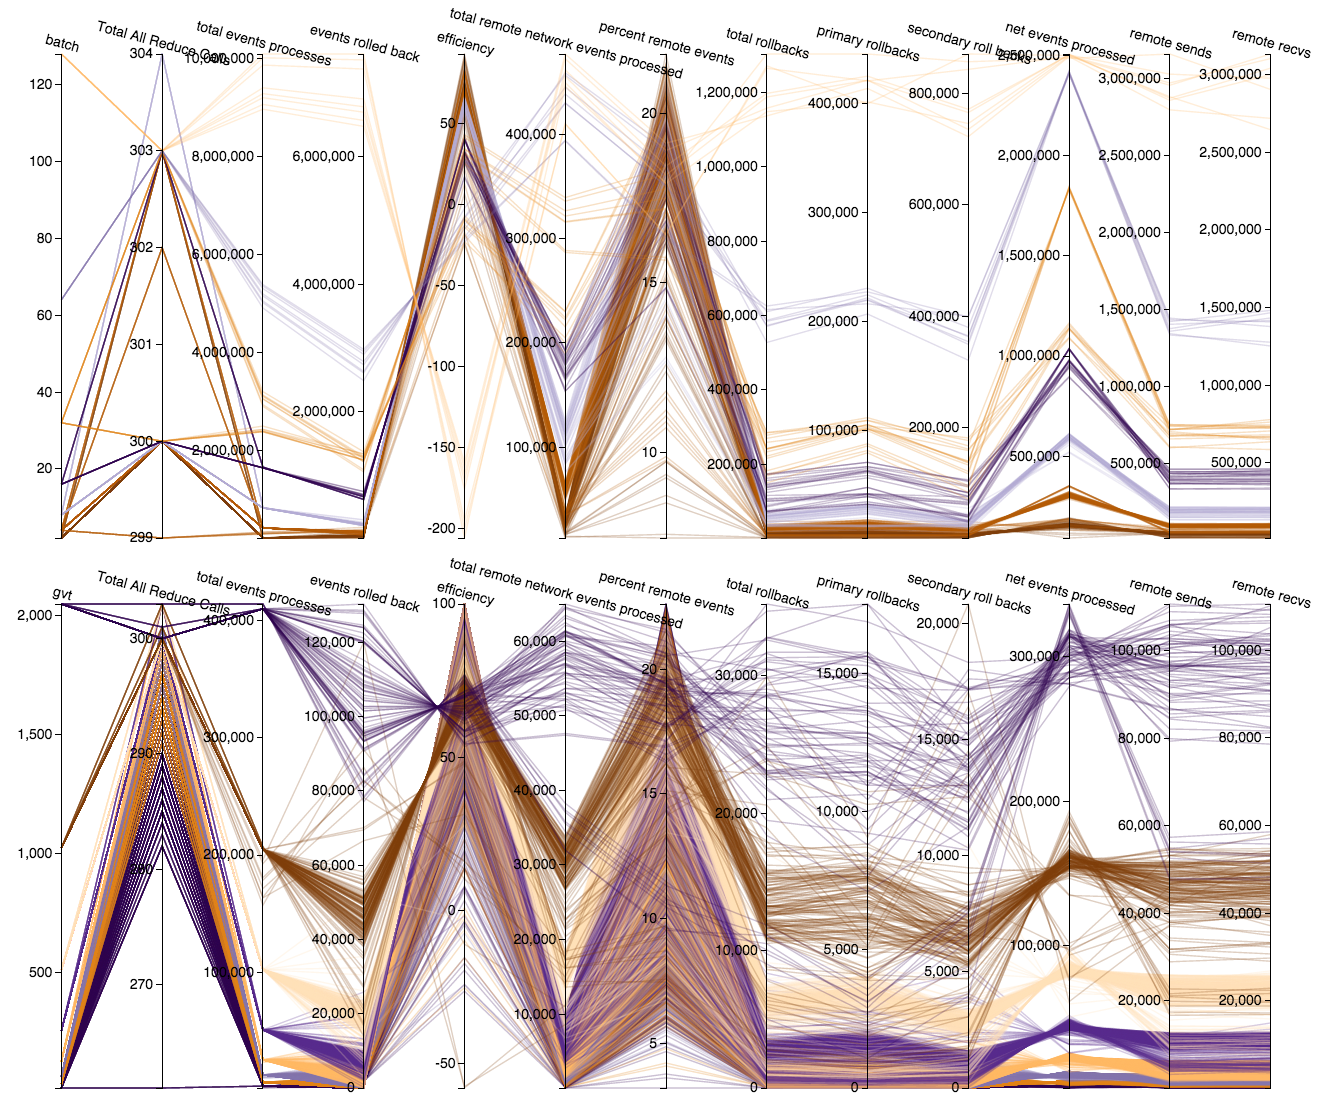
\includegraphics[width=7in]{figures/blind-white.png}
\caption{Parallel Coordinates graph for runs with various batch values}
\label{fig:batch}
\end{figure}
\begin{figure}[ht]
\centering
	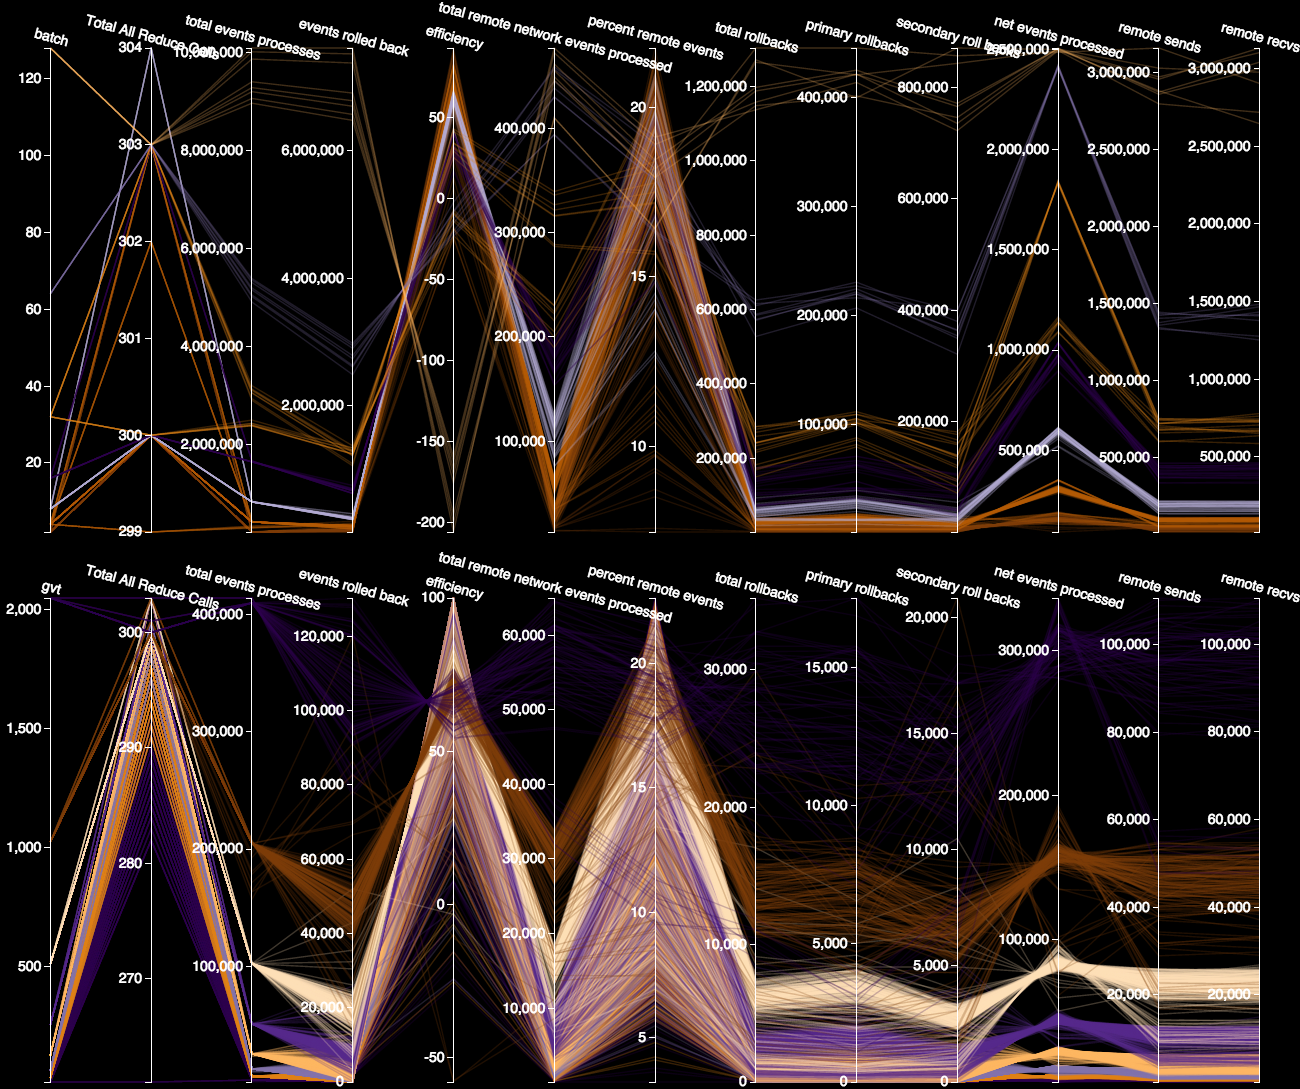
\includegraphics[width=7in]{figures/blind-black.png}
\caption{Parallel Coordinates graph for runs with various gvt-interval values}
\label{fig:gvt}
\end{figure}

\section{Visualization Tool Review}
%A brief review of the tool you used to create the visualizations.
As mentioned before, we used Plotly to generate the area plot visualizations of the dataset. Plotly is a web based utility that also has support and APIs for non web based applications such as Excel, Matlab and programming languages like R and python. Overall, Plotly is a very user friendly and easy to use tool for creating relatively dynamic visualizations. The interface is very similar to an excel worksheet and allows you to import data from file or create and manipulate data within the worksheet. Plotly also has a large selection of visualization types from ugly simple pie charts to complex heat maps and large sets of interaction capabilites. The Plotly vis tool also appears to have no issues with handling large data sets. The one downfall for the software is the control over the visualizations. After you select the type of visualization you want, the amount of customization is very limited. Perhaps there is more customization if you use the API with python or another language. 

The d3.parcoords.js library used made the creation of the parallel coordinates graph very simple.  Before finding this library, we tried to edit an example that used d3.js only, but it was very difficult for us to figure out how to get the various colors set for each grouping of batch or gvt\_interval data points.  Once we found this library, it was very simple to add in color, as well as the interactive aspects (axis shuffling and selection of a subset of the data).  However, we still had difficulty with trying to change the scales of the axes.  The current setup just bases it on the data, but it would be more helpful to match the axes between the two different graphs so that each metric has the same scale on both graphs.  

% Bibliography
\bibliographystyle{abbrv}
\bibliography{hw5}

\end{document}


%\begin{figure}[!ht]
%     \centering
%     \subfloat[][twopi]{\epsfig{file=figures/MMS7-3-17.png, height=2.2in, width=4.80in}\label{vis-100-1}}\\
%     \subfloat[][dot]{\epsfig{file=figures/MMS7-3-12.png, height=2.0in, width=3.00in}\label{vis-100-2}}
%     \subfloat[][circo]{\epsfig{file=figures/MMS7-3-circo.png, height=2.0in, width=3.0in}\label{vis-100-3}}\\
%     \caption{Visualizations of the class social network data using a collection of Graphviz graph drawing programs. Red lines represent "before RPI" connections, blue represent "lived with" connections and black represent "Data Structures" connections. }
%     \label{vc-occupancy}
%\end{figure}

%\begin{figure}[!h]
%\centering
%\epsfig{file=figures/storyboard.jpg, width=5.5in}
%\caption{Storyboard showing the desired layout and interaction of the network visualization tool in D3.}
%\label{good}
%\end{figure}